\documentclass[a4paper,11pt]{article}


\usepackage{alphabeta}
\usepackage{graphicx}

\usepackage[utf8x]{inputenc}

\usepackage{amsfonts , amssymb , amsmath}
\usepackage{float}
\usepackage{multirow}
\usepackage{amsmath}

\title{Αριθμητική Ανάλυση - 2η Εργασία}
\author{Ονοματεπώνυμο: Νικόλαος Ιλαρίδης \\ ΑΕΜ: 4524}
\date{\today}

\begin{document}
	\maketitle
	
	\section{Πέμπτη Ασκηση}
	\begin{enumerate}
		\item[\textbf{(α)}] \emph {\textbf{Πολυωνυμική προσέγγιση}}
		\vspace{2cm}
		\begin{center}
			Στο αρχειο '\textbf{lagrange.py}' που βρισκεται στον φακελο 'Ex5' προσεγγιζω πολυωνυμικα την συναρτηση \textbf{sin(x)} και πιο συγκεκριμενα χρησιμοποιω το πολυωνυμο lagrange . Αρχικα οριζω καποιες μη ομοιομορφα κατανεμημενες γωνιες στο διαστημα \textbf{[-π,π]} οι οποιες θα χρησιμοποιηθουν απο την συναρτηση lagrange για τον υπολογισμου του πολυωνυμου ενω στην συνεχεια θα δοκιμαστει η ακριβεια του με 200 νεες γωνιες στο ιδιο διαστημα. Εν τελει η συναρτηση lagrange επιστρεφει ενα πινακα result μεγεθους n ο οποιος περιεχει τις προσεγγισεις για την ζητουμενη συναρτηση με τις οποιες υπολογιζουμε και το θεωριτικο σφαλμα του αλγοριθμου μας υπολογιζοντας την διαφορα της προσεγγισης με την τιμη που δινει η συναρτηση sin(x) του πακετου \underline{numpy} της python , το οποιο και αποθηκευεται στον πινακα error . Παρακατω παραθετω ορισμενες απο τις 200 γωνιες που εγιναν οι δοκιμες ακριβειας του αλγοριθμου καθως και το διαγραμμα σφαλματων το οποιο σχεδιασα με την χρηση της βιβλιοθηκης  \underline{matplotlib.pyplot} .
		\end{center}

		\begin{center}
			\emph{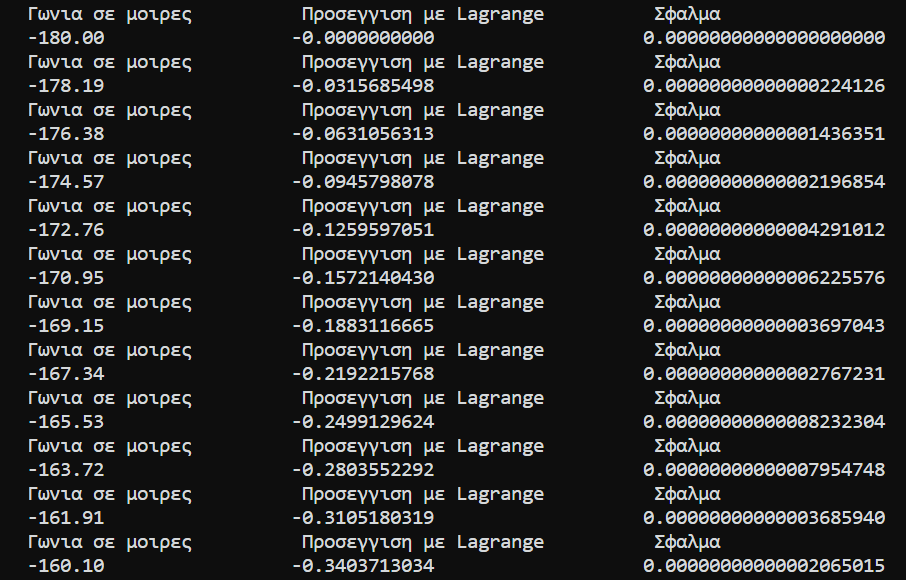
\includegraphics[scale=0.5]{lagrange.png}}
		\end{center}
		\begin{center}
			\emph{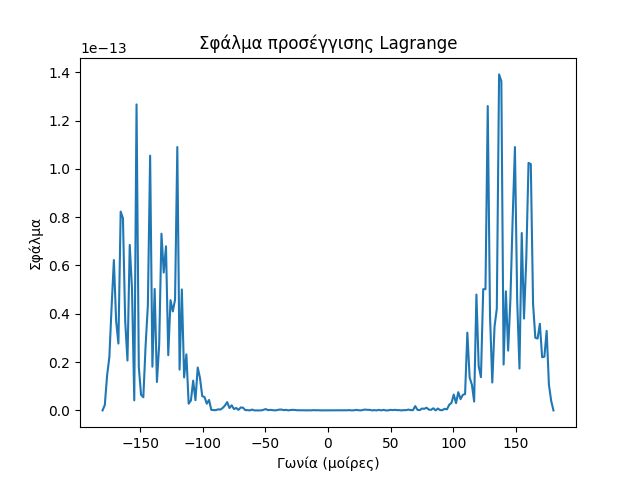
\includegraphics[scale=0.75]{lagrangerror.png}}
		\end{center}
		\begin{center}
			Παρατηροντας τα αποτελεσματα του προγραμματος παρατηρουμε οτι πετυχαινει αρκετα μεγαλη ακριβεια, και μαλιστα στις περισσοτερες τιμες εξασφαλιζει ακριβεια \textbf{13 δεκαδικων} ψηφιων . 
		\end{center}
		\vspace{0.7cm}
		\item[\textbf{(β)}] \emph {\textbf{Splines}}
		\begin{center}
			Για την υλοποιηση της μεθοδου \textbf{splines} χρησιμοποιησα ενα αλγοριθμο τον οποιο βρηκα απο ενα βιβλιο αριθμητικης αναλυσης στο διαδικτυο , τα βηματα του οποιου παραθετω παρακατω. 
		\end{center}
		\begin{center}
			\emph{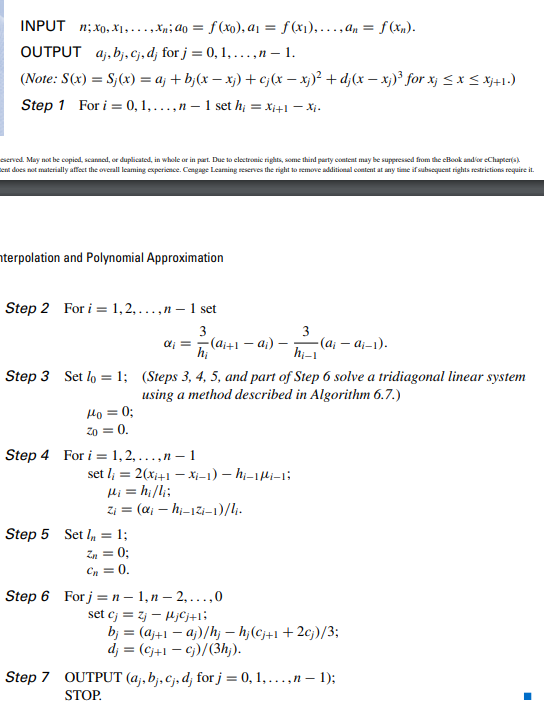
\includegraphics[scale=0.75]{splinesAlgorithm.png}}
		\end{center}
		\begin{center}
			Ωστοσο τα βηματα 3,4 και 5 που λυνουν το γραμμικο συστημα τα εχω αντικαταστησει χρησιμοποιοντας αναλυση \textbf{PA=LU} την οποια ειχα υλοποιησι στην προηγουμενη εργασια και εχω προσθεσει τον κωδικα στην αρχη του προγραμματος. Επισης οπως και στην προηγουμενη μεθοδο χρησιμοποιουνται οι ιδιες 10 γωνιες για την προσεγγιση της συναρτησης και στην συνεχεια δοκιμαζεται η ακριβεια σε αλλες 200 γωνιες.
		\end{center}
		\begin{center}
			\emph{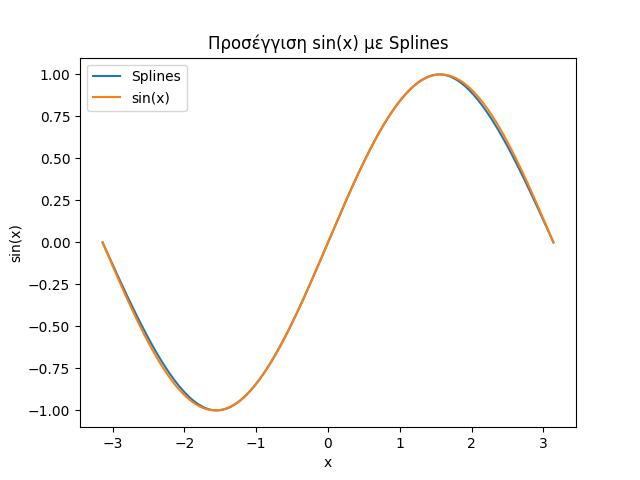
\includegraphics[scale=0.75]{splines.png}}
		\end{center}
		\begin{center}
			Η \underline{πορτοκαλι γραμμη} που φαινεται στο διαγραμμα ειναι η γραφικη παρασταση της \textbf{sin(x)} και με \underline{μπλε χρωμα} εμφανιζεται η προσεγγιση της.
		\end{center}
		\begin{center}
			\emph{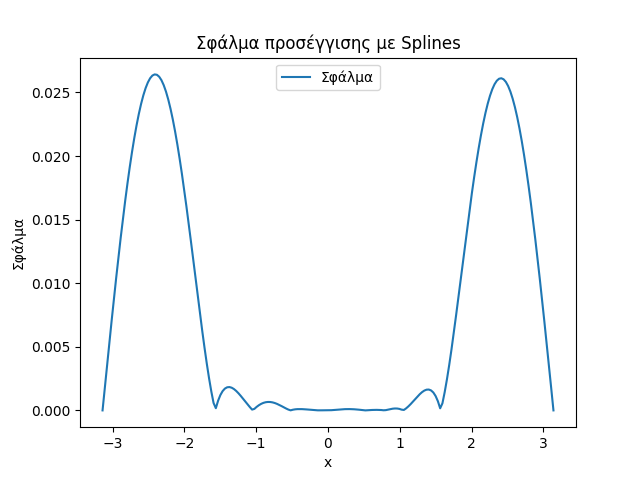
\includegraphics[scale=0.75]{splinesError.png}}
		\end{center}
		\begin{center}
			Το διαγραμμα του σφαλματος φαινεται παρομμοιο με το αντιστοιχο με Lagrange ωστοσο η μεθοδος αυτη πετυχαινει ακομα \underline{μεγαλυτερη ακριβεια}, γεγονος που απεικονιζεται και στο διαγραμμα.
		\end{center}
		
		\item[\textbf{(γ)}] \emph {\textbf{Ελαχιστα Τετραγωνα}}
		\begin{center}
			Για την μεθοδο αυτη αρχικα προσεγγισα την συναρτηση με πολυωνυμο πρωτου βαθμου , αλλα παρατηρησα οτι οσο μεγαλωνει ο βαθμος του πολυωνυμου εχουμε μεγαλυτερη ακριβεια στην προσεγγιση της συναρτησης. Ετσι αποφασισα να την υλοποιησω με πολυωνυμο 7ου βαθμου, με τις ιδιες 10 γωνιες που χρησιμοποιηθηκαν και για τις αλλες μεθοδους. Για να βρω το πολυωνυμο πρεπει να λυσουμε την εξης εξισωση : $$Α^{Τ}Αx' = A^{T}b$$   Ετσι στο προγραμμα που υπολογιζω τον πινακα Α και στην συνεχεια τον αναστροφο του , ενω αμεσως μετα προκειμενου να φτασω την εξισωση στην μορφη που θελουμε πολλαπλασιαζω τον πινακα Α με τον αναστροφο του και μετα πολλαπλασιαζω τον ανεστραμενο με τον πινακα που περιεχει τις τιμες του ημ(χ). Ετσι πρεπει να λυσω το γραμμικο συστημα που εμφανιζεται . Για την επιλυση του χρησιμοποιω αναλυση PA=LU την οποια εχω υλοποιησει σε προηγουμενη εργασια. 
		\end{center}
		\begin{center}
			Μερικες απο τις 200 προσεγγισεις με την μεθοδο ελαχιστων τετραγωνων: 
		\end{center}
		\begin{center}
			\emph{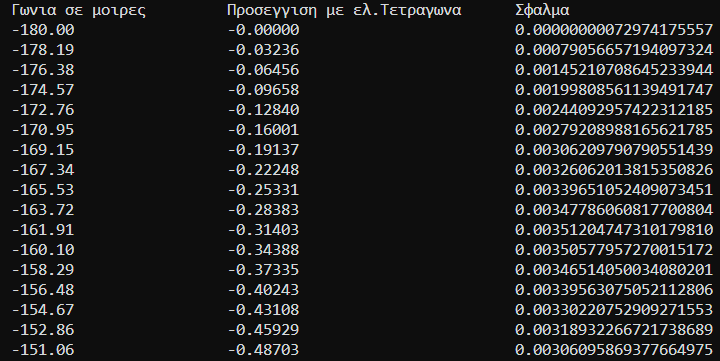
\includegraphics[scale=0.75]{leastSquares.png}}
		\end{center}
		\begin{center}
			\emph{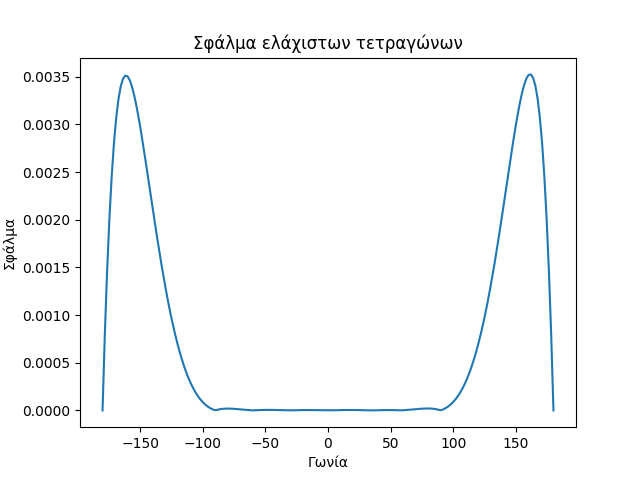
\includegraphics[scale=0.75]{leastSquaresError.png}}
		\end{center}
		\begin{center}
			Οπως βλεπουμε ακομη μια φορα το διαγραμμα των σφαλματων ειναι παρομοιο, ωστοσο η ακριβεια που πετυχαινουμε ειναι σαφως μικροτερη (3 δεκαδικα ψηφια) γεγονος ομως που μπορει να βελτιωθει οσο μεγαλωνει ο βαθμος του πολυωνυμου. 
		\end{center}
	\end{enumerate}
	\section{Εκτη Ασκηση}
	\begin{enumerate}
		\item[\textbf{(α)}] \emph {\textbf{Simpson}}
		\begin{center}
			Στο αρχειο \textbf{simpson.py} που βρισκεται στον φακελο Ex6 προσεγγιζω το ολοκληρωμα της \textbf{sin(x)} στο διαστημα \textbf{[0,π/2]} με την μεθοδο simpson . Πιο συγκεκριμενα καθως ζηταει η εκφωνηση να κανω χρηση 11 σημειων θα σπασω το αρχικο μου διαστημα σε 10 υποδιαστηματα συμφωνα με τον τυπο $$x_i = x_0+k*(b-a)/n$$ Στην συνεχεια συμφωνα με τον παρακατω τυπο υπολογιζω τα 2 αθροισματα καθως και τις τιμες στα ακρα για να προσεγγισω το ολοκληρωμα $$\int_{a}^{b}f(x)dx\cong\dfrac{b-a}{3N}(f(x_0) + f(x_N) + 2\sum_{i=1}^{\dfrac{N}{2}-1}f(x_{2i}) + 4\sum_{i=1}^{\dfrac{N}{2}-1}f(x_{2i-1}))$$
		\end{center}
		\begin{center}
			Εφοσον εχει γινει η προσεγγιση μενει μονο ο υπολογισμος του σφαλματος προσεγγισης τοσο θεωριτικα οσο και αριθμητικα.Τα αποτελεσματα του δικου μου κωδικα φαινονται παρακατω πετυχαινοντας ακριβεια \underline{5 δεκαδικων} .
		\end{center}
		\begin{center}
			\emph{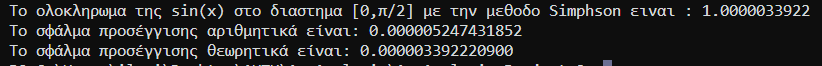
\includegraphics[scale=0.55]{simpson.png}}
		\end{center}
		
		\item[\textbf{(β)}] \emph {\textbf{Μεθοδος Τραπεζιου}}
		\begin{center}
			Οπως και στην προηγουμενη μεθοδο στην αρχη σπαμε το διαστημα [0,π/2] σε 10 υποδιαστημτα. Στην συνεχεια βρισκουμε τις τιμες $f(x_i)$ , i= 0,...,N , τις αθροιζουμε και πολλαπλασιαζουμε *2 , ενω τελος πολλαπλασιαζουμε το γενικο αθροισμα με το \textbf{interval = (b-a)/n} δια 2 . 
		\end{center}
		\begin{center}
			Οπως και στην προηγουμενη μεθοδο μενει να υπολογισουμε το σφαλμα \underline{θεωρητικα} και \underline{αριθμητικα} χρησιμοποιοντας τον καταλληλο τυπο για το αριθμητικο σφαλμα και υπολογιζοντας την διαφορα της προσεγγισης με το κανονικο ολοκληρωμα για το θεωρητικο σφαλμα . Τα αποτελεσματα παραθετονται παρακατω .
		\end{center}
		\begin{center}
			\emph{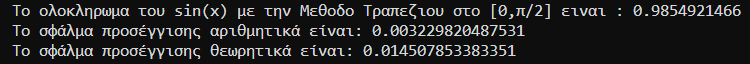
\includegraphics[scale=0.55]{trapezium.png}}
		\end{center}
		\begin{center}
			Παρατηρουμε οτι με αυτη την μεθοδο εχουμε μεγαλυτερο σφαλμα σε σχεση με την Simpson καθως πετυχαινουμε ακριβεια μονο \underline{2 δεκαδικων} για το αριθμητικο σφαλμα και \underline{1 για το θεωρητικο}.
		\end{center}
	\end{enumerate}
	
	\section{Εβδομη Ασκηση}
	
	\begin{center}
		Για την Ασκηση 7 επελεξα να χρησιμοποιησω τα κρυπτονομισματα \textbf{BTC} και \textbf{SOL} και η ημερομηνια γενεθλιων μου ειναι \underline{20 Οκτωβριου} , αρα προσεγγιζω τις τιμες των νομισματων για τις μερες \underline{21 εως 25 Οκτωβριου 2023}.
	\end{center}
	\begin{center}
		Η μεθοδος που χρησιμοποιουμε ειναι ιδια με αυτη της ασκησης 5 στο 3ο μερος με την διαφορα οτι εδω η εκφωνηση ζητα αυστηρα με πολυωνυμο \textbf{2ου 3ου και 4ου βαθμου}, οποτε δεν θα σταθω τοσο στην μεθοδο αλλα στα αποτελεσματα της προσεγγισης. 
	\end{center}
	\begin{center}
		Λυνοντας την ασκηση παρατηρησα επισης οτι καθως προκειται για προβλεψη και οχι προσεγγιση της τιμης των νομισματων μεγαλωνοντας τον βαθμο του πολυωνυμου δεν αυξανεται απαραιτητα και η ακριβεια οπως γινοταν στην ασκηση 5.
	\end{center}
	\begin{center}
		Παρακατω παραθετω τα αποτελεσματα των αλγοριθμων μου παραλληλα με την πραγματικη τιμη κλεισιματος του νομισματος εκεινης της μερας. 
	\end{center}
	\begin{center}
	\textbf{	2ου Βαθμου Πολυωνυμο }
	\end{center}
	\begin{center}
		\emph{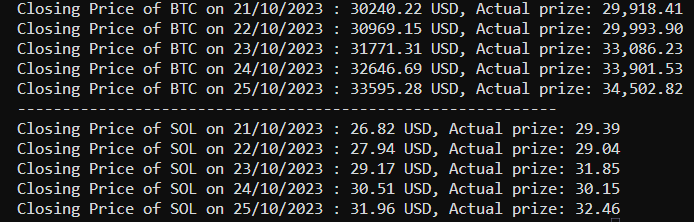
\includegraphics[scale=0.75]{ex7_2.png}}
	\end{center}
	\begin{center}
		\textbf{	3ου Βαθμου Πολυωνυμο }
	\end{center}
	\begin{center}
		\emph{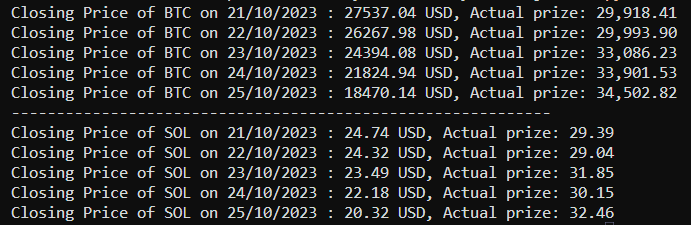
\includegraphics[scale=0.75]{ex7_3.png}}
	\end{center}
	\begin{center}
		\textbf{	4ου Βαθμου Πολυωνυμο }
	\end{center}
	\begin{center}
		\emph{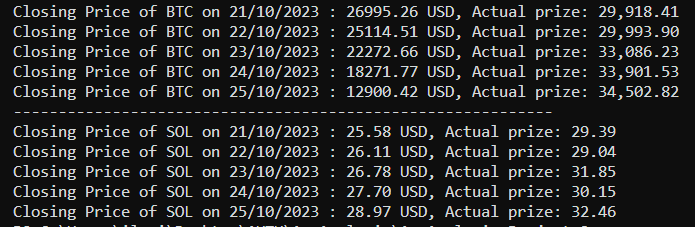
\includegraphics[scale=0.75]{ex7_4.png}}
	\end{center}
	\begin{center}
		Παρατηρουμε οτι οσο μεγαλωνει το διαστημα που θελουμε να κανουμε την προβλεψη , μεγαλωνει και το σφαλμα . Αυτο μπορει να συμβαινει γιατι για την κατασκευη του πολυωνυμου εχουν χρησιμοποιηθει μονο 10 τιμες , ενω τελος παρατηρουμε να μεγαλωνει το σφαλμα οσο μεγαλωνει και ο βαθμος του πολυωνυμου σε αντιθεση με την Ασκηση 5
	\end{center}
\end{document}